\begin{figure}[ht]
\centering
% Thesis-wide categorical color palette
% Usage: % Thesis-wide categorical color palette
% Usage: % Thesis-wide categorical color palette
% Usage: \input{figures/palette} in any figure file
%
% Muted primary colors -- print-friendly, visually distinct.
% Inspired by Cooper Union's red/blue primaries, softened for
% academic figures. Use palA-palC for data series in scatter
% plots, line charts, bar charts, etc.

\definecolor{palA}{HTML}{1F77B4}   % Tableau blue
\definecolor{palB}{HTML}{D62728}   % Tableau red
\definecolor{palC}{HTML}{2CA02C}   % Tableau green
 in any figure file
%
% Muted primary colors -- print-friendly, visually distinct.
% Inspired by Cooper Union's red/blue primaries, softened for
% academic figures. Use palA-palC for data series in scatter
% plots, line charts, bar charts, etc.

\definecolor{palA}{HTML}{1F77B4}   % Tableau blue
\definecolor{palB}{HTML}{D62728}   % Tableau red
\definecolor{palC}{HTML}{2CA02C}   % Tableau green
 in any figure file
%
% Muted primary colors -- print-friendly, visually distinct.
% Inspired by Cooper Union's red/blue primaries, softened for
% academic figures. Use palA-palC for data series in scatter
% plots, line charts, bar charts, etc.

\definecolor{palA}{HTML}{1F77B4}   % Tableau blue
\definecolor{palB}{HTML}{D62728}   % Tableau red
\definecolor{palC}{HTML}{2CA02C}   % Tableau green

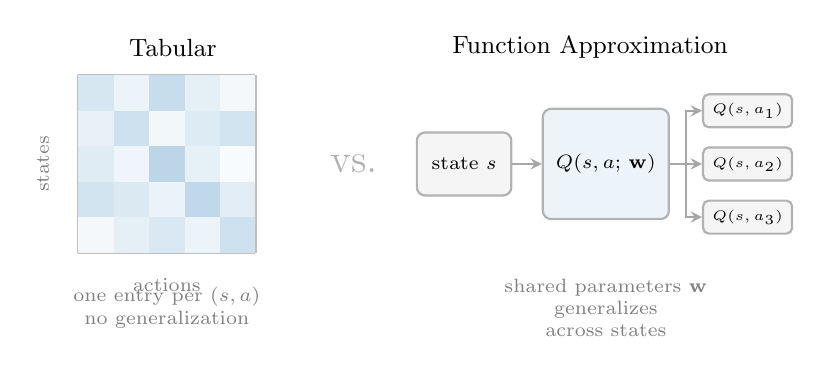
\begin{tikzpicture}[
    arr/.style={->, thick, >=stealth, black!35},
    lbl/.style={font=\small},
    sublbl/.style={font=\scriptsize, text=black!50},
]

% --- Tabular (left) ---
\node[lbl] at (1.2, 2.6) {Tabular};

% Q-table grid
\draw[thick, black!25] (0, 0) grid[step=0.45] (2.25, 2.25);

% Row/column labels
\node[sublbl, rotate=90, anchor=south] at (-0.25, 1.125) {states};
\node[sublbl, anchor=north] at (1.125, -0.2) {actions};

% Fill a few cells to suggest values
\foreach \x/\y/\c in {
    0/4/18, 1/4/8, 2/4/25, 3/4/12, 4/4/5,
    0/3/10, 1/3/22, 2/3/6, 3/3/15, 4/3/20,
    0/2/14, 1/2/7, 2/2/30, 3/2/11, 4/2/3,
    0/1/20, 1/1/16, 2/1/9, 3/1/28, 4/1/13,
    0/0/5, 1/0/12, 2/0/17, 3/0/8, 4/0/22
} {
    \fill[palA!\c] ({\x*0.45}, {\y*0.45})
        rectangle ({(\x+1)*0.45}, {(\y+1)*0.45});
}

% "one entry per (s, a)" label
\node[sublbl, text width=2.5cm, align=center] at (1.125, -0.7)
    {one entry per $(s, a)$\\no generalization};

% --- Arrow ---
\node[font=\Large, text=black!30] at (3.5, 1.125) {vs.};

% --- Function approximation (right) ---
\node[lbl] at (6.5, 2.6) {Function Approximation};

% State input
\node[draw=black!30, thick, rounded corners=3pt,
      minimum width=1.2cm, minimum height=0.8cm,
      font=\scriptsize, fill=black!4]
    (state) at (4.9, 1.125) {state $s$};

% Network box
\node[draw=black!30, thick, rounded corners=3pt,
      minimum width=1.6cm, minimum height=1.4cm,
      font=\scriptsize, fill=palA!8, align=center]
    (net) at (6.7, 1.125) {$Q(s, a;\, \mathbf{w})$};

% Q-value outputs
\node[draw=black!30, thick, rounded corners=2pt,
      minimum width=0.9cm, minimum height=0.4cm,
      font=\tiny, fill=black!4]
    (q1) at (8.5, 1.8) {$Q(s, a_1)$};
\node[draw=black!30, thick, rounded corners=2pt,
      minimum width=0.9cm, minimum height=0.4cm,
      font=\tiny, fill=black!4]
    (q2) at (8.5, 1.125) {$Q(s, a_2)$};
\node[draw=black!30, thick, rounded corners=2pt,
      minimum width=0.9cm, minimum height=0.4cm,
      font=\tiny, fill=black!4]
    (q3) at (8.5, 0.45) {$Q(s, a_3)$};

\draw[arr] (state) -- (net);
\draw[arr] (net.east) -- ++(0.2, 0) |- (q1.west);
\draw[arr] (net.east) -- (q2.west);
\draw[arr] (net.east) -- ++(0.2, 0) |- (q3.west);

% Label
\node[sublbl, text width=2.8cm, align=center] at (6.7, -0.7)
    {shared parameters $\mathbf{w}$\\generalizes across states};

\end{tikzpicture}
\caption{Tabular Q-learning stores one value per state--action pair.
  Function approximation maps states to Q-values through shared
  parameters, enabling generalization.}
\label{fig:table-vs-network}
\end{figure}
